

\section{AdHoc Problems}

\begin{frame}
  \centering
  {\huge
    Week 1 -- Part 3: AdHoc Problems
  }
\end{frame}

\begin{frame}
  \frametitle{What are Ad-hoc problems?}

  \emph{Ad-hoc} is an expression used to mean something used for a single purpose. In programming challenges, an \structure{ad-hoc problem} is a simple problem that you can solve by simply following the instructions.
  \bigskip

  Although ad-hoc problems are simple, it is good to practice them seriously, as we can learn skills that are useful for more complex problems too:
  \bigskip

  \begin{itemize}
    \item Extracting important information from the problem text;
    \item Understanding the input and output;
    \item Generating debug and worst case data;
    \item Analysing problems;
  \end{itemize}
  \bigskip

  In this lecture, we will see some hints that will be useful for the
  entire course.
\end{frame}

\section{Problem Analysis}
\subsection{Revisiting the 3n+1 problem}
\begin{frame}{Revisiting the 3n+1 problem}
  Let's revisit the 3n+1 problem, that we introduced in the beginning of this class.
  \bigskip

  This is a great problem because it is very simple, but you still need to be careful when implementing the solution.
\end{frame}

\begin{frame}[fragile]{Revisiting the 3n+1 problem}{Problem outline}

  \begin{block}{}
    Calculate the {\bf Maximum Cycle Length} between any two numbers $i$ and $j$.
  \end{block}
  \bigskip

\begin{verbatim}
Cycle of (n)
1. print n
2. if n == 1 then STOP
3. if n is odd then n = 3n + 1
4. else n = n/2
5. GOTO 2

Example: Cycle of (22)
22 11 34 17 52 26 13 40 20 10 5 16 8 4 2 1

Size: 16
\end{verbatim}
\end{frame}

\begin{frame}[fragile]
  \frametitle{A simple solution for the 3n+1 problem}
\begin{verbatim}
while true:
  try:
    line = input()
    max = 0
    tk = line.split()
    i, j = int(tk[0]), int(tk[1])
    for n in range(i, j+1):
      count = 1
      while n != 1:
        if n % 2 == 1: n = 3 * n + 1
        else: n = n / 2
        count += 1
      if count > max: max = count
    print (line, max)
  except EOFError: break
\end{verbatim}
\end{frame}

\begin{frame}{A Simple Solution has a Simple problem}

  \begin{itemize}
    \item If you submit the simple solution in the previous slide, you will receive the result \alert{Wrong Answer} from the judge.
    \bigskip

    \item You look at the example input and output, and your program gets the correct solution for all the sample input!
    \item You even try a few more values of $i$ and $j$ to make sure.
    \bigskip

    \item What is wrong with the simple solution? (Answer in the next slide)
  \end{itemize}
\end{frame}

\begin{frame}[fragile]
  \frametitle{Trick Hidden Inputs}

  \begin{itemize}
    \item The first solution solves all the sample input correctly, but
    there are some inputs that can cause problems.
    \bigskip

    \item For example, think of this input: \alert{$i = 20, j = 10$}
    \item The output will be nothing!
    \bigskip

    \item Here is the code that causes this problem:
\begin{verbatim}
for x in range(i, j+1):   <-- Error is here!
  ...
  print (line, max)
\end{verbatim}
    \bigskip

    \item But in the input there are no examples with "$i > j$" is this
    allowed?
  \end{itemize}
\end{frame}

\begin{frame}{Trick Hidden Inputs}{Reading the input carefully}
  The problem page has a description that include an {\bf input} section:

  \begin{block}{Input Description}
    The input will consist of a series of \alert{pairs of integers} i and j, one pair of integers per line. All integers will be \alert{less than 10,000 and greater than 0.}

    \bigskip

    You should process all pairs of integers and for each pair determine the maximum cycle length over \alert{all integers between and including i and j}.
    \bigskip

    You can \alert{assume that no operation overflows a 32-bit integer}.
  \end{block}
  \bigskip

  In the input section, there is no rule that forces $j > i$!
  \medskip

  If it is not forbidden by the rules, then maybe it will happen!
\end{frame}

\begin{frame}{Trick Hidden Inputs}{General Rules}

  \begin{itemize}
    \item First rule of Programming Challenges:\\
      \hspace{1cm}\alert{If it is not written, assume the worst case}
    \bigskip

    \item Some common tricky inputs to be careful:
    \begin{itemize}
      \item A number is negative; a number is zero; a number is maximum;
      \item The input is out of order (or in order!);
      \item The input is repeated;
      \smallskip

      \item A graph is unconnected; a graph is fully connected;
      \item Lines are parallel; points are in the same place;
      \item An area is 0; an angle is 0;
      \smallskip

      \item The input is very long;
      \item The input is very short;
    \end{itemize}
    \bigskip

    \item If it is not against the rules, it may (will?) happen;
    \item This first rule is also important for the real world!
  \end{itemize}
\end{frame}

\begin{frame}[fragile]{Problem 3n+1}{A fixed solution for the input}
\begin{verbatim}
while true:
  try:
    line = input()
    max = 0
    tk = line.split()
    i, j = int(tk[0]), int(tk[1])
    for n in range(min(i, j), max(i, j)+1): # FIXED!
      count = 0
      while n != 1:
        if n % 2 == 1: n = 3 * n + 1
        else: n = n / 2
        count += 1
      if count > max: max = count
    print (line, max)
  except EOFError: break
\end{verbatim}
\end{frame}

\begin{frame}
  \frametitle{This solution has a problem too!}
  \begin{itemize}
    \item This time we are sure that the solution is correct for all inputs;
    \item But you still do not get "accepted" in the online judge...
    \bigskip

    \item Now the judge says \alert{"Time limited exceeded"}.
    \bigskip

    \item What happened? (Think a little bit on this one)
  \end{itemize}
\end{frame}

\begin{frame}[fragile]
  \frametitle{Solution 2: Be careful of computing costs!}

    \begin{block}{Input Description}
    All integers will be \alert{less than 10,000 and greater than 0.}
    \bigskip

    You can \alert{assume that no operation overflows a 32-bit integer}.
    \end{block}
    \bigskip

    \begin{itemize}
      \item What happens when the input is \alert{minimum and maximum}?
\begin{verbatim}
1 10000 262
\end{verbatim}
      \bigskip

      \item A sequence with 262 steps does not seem very long.
      \item But remember we calculate \alert{all} sequences between 1, 10000!
      \item Estimate the cost: $10000 \times 262 \approx 2,000,000$ steps!
      \bigskip

      \item This is one query. The input can have repeated queries!
    \end{itemize}
\end{frame}

\begin{frame}[fragile]
  \frametitle{Avoiding repeated work}

  \begin{itemize}
    \item Think about the cycle calculation (let's call it A(n));
\begin{verbatim}
A(22):  22 11 34 17 52 26 13 40 20 10 5 16 8 4 2 1
A(11):  11 34 17 52 26 13 40 20 10 5 16 8 4 2 1
A(17):  17 52 26 13 40 20 10 5 16 8 4 2 1
A(13):  13 40 20 10 5 16 8 4 2 1
A(10):  10 5 16 8 4 2 1
A(8) :  8 4 2 1
\end{verbatim}
    \bigskip

    \item Can we avoid all this recalculation?
  \end{itemize}

  \begin{block}{Good Technique: Memoization}
    Store the result of a function that we know will be calculated again in the future. \structure{This is useful for many problems!}
  \end{block}
\end{frame}

\begin{frame}[fragile]{Avoiding Repeated Work}{Memoization Idea}
  To implement \alert{Memoization}, we use a table or dictionary to store partial results.
\begin{verbatim}
  table = {}
  table[1] = 1
  def A(n):
    if n in table.keys(): return table[n]
    else:
      if n % 2 == 1: table[n] = 1 + A(3*n + 1)
      else: table[n] = 1 + A(n/2)
    return table[n]
\end{verbatim}
In a future class, we will focus on \alert{Dynamic Programming}, which generalizes this technique.
\end{frame}

% \section{How to Solve Problems}
% \subsection{Programming Challenge Workflow}
% \begin{frame}
%   \frametitle{A Programming Challenge Workflow}
%
%   \begin{center}
%     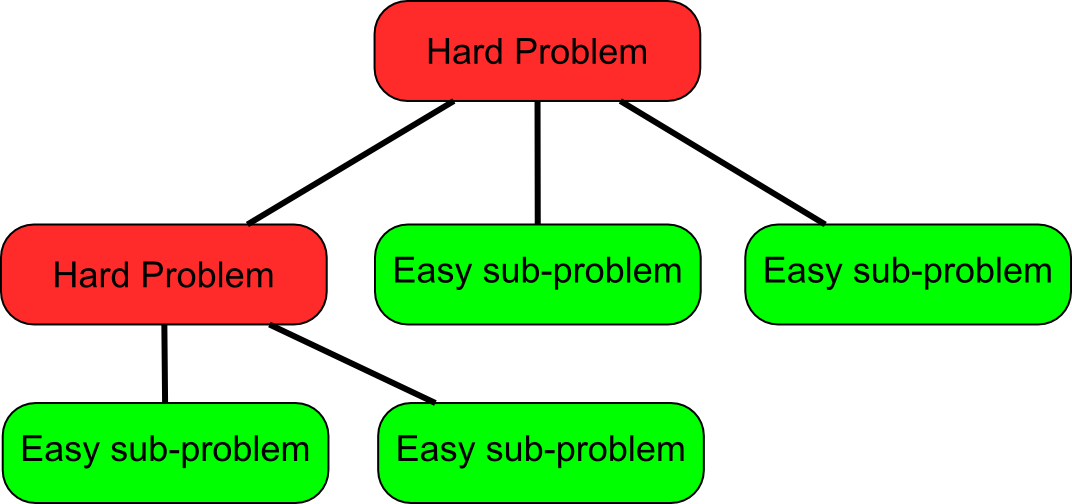
\includegraphics[width=0.5\textwidth]{../img/breakingtheproblem}
%   \end{center}
%
%   Trick to solve problems without bugs: Break the problem down
%   \bigskip
%
%   \begin{itemize}
%   \item How to calculate the function $A()$;
%   \item Imagine the worst possible cases ($i > j$);
%   \item Calculate cost of solution;
%   \item Improve speed with memoization;
%   \end{itemize}
% \end{frame}

\section{Programming Challenge Workflow}
\begin{frame}
  \frametitle{A Programming Challenge Workflow}

  When solving a programming challenge, you want to follow
  these common steps:
  \bigskip

  \begin{itemize}
  \item Task 1: Read the problem description;
  \item Task 2: Read the input/output;
  \item Task 3: Think about the algorithm;
  \item Task 4: Write the Code;
  \item Task 5: Test the program on example data;
  \item Task 6: Test the program on hidden data;
  \end{itemize}
\end{frame}


\subsection{Reading The Problem}
\begin{frame}
  \frametitle{Task 1: Understanding the Problem Description}

  Reading and understanding the problem is very important! Try to
  understand completely the problem before starting to program.
  \bigskip

  \begin{block}{General Tips}
  \begin{itemize}
  \item Find the \alert{rules} of the problem, separate from the \alert{story};
  \item Sometimes it is easy to read the input/output part first;
  \item Problems with a lot of \alert{story} are usually not very hard.;
\end{itemize}
  \end{block}

  \begin{alertblock}{Reading English is Hard!}
    \begin{itemize}
      \item Don't worry!
      \item Focus on the keywords;
      \item Understanding a little English is important for CS!
      \item Get help from professor Google Translate;
    \end{itemize}
  \end{alertblock}
\end{frame}

\begin{frame}
  \frametitle{Example: Problem 11559 -- Event Planning}

  {\smaller
  \begin{alertblock}{Story:}
    As you didn't show up to the yearly general meeting of the Nordic
    Club of Pin Collectors, you were unanimously elected to organize
    this years excursion to Pin City.  You are free to choose from a
    number of weekends this autumn, and have to find a suitable hotel
    to stay at, preferably as cheap as possible.
  \end{alertblock}

  \begin{exampleblock}{Rules}
    You have some \structure{\underline{constraints}}: The total
    \structure{\underline{cost}} of the trip must be within
    \structure{\underline{budget}}, of course. All participants
    \structure{\underline{must}} stay at the same hotel, to avoid last years
    catastrophe, where some members got lost in the city, never being seen
    again.
  \end{exampleblock}}

  How do you tell the difference between Story and Rules? Look for the keywords!
  \bigskip

  {\bf Keywords:} constraints, minimum, maximum, cost, rules, number, etc...
\end{frame}

\begin{frame}
  \frametitle{Hints for Reading Problems}

  \begin{columns}
    \column{0.7\textwidth}
    {\small
    \begin{itemize}
    \item First, look at the \structure{sample input and output};
    \item Write the key ideas on paper
    \item Use the Paper: mark keywords;
    \item Use the Paper: cut flavor;
    \item \alert{Read the problem again!};
    \item \alert{Do not begin programming until you understand the problem!}
    \end{itemize}
    }
    \column{0.3\textwidth}
    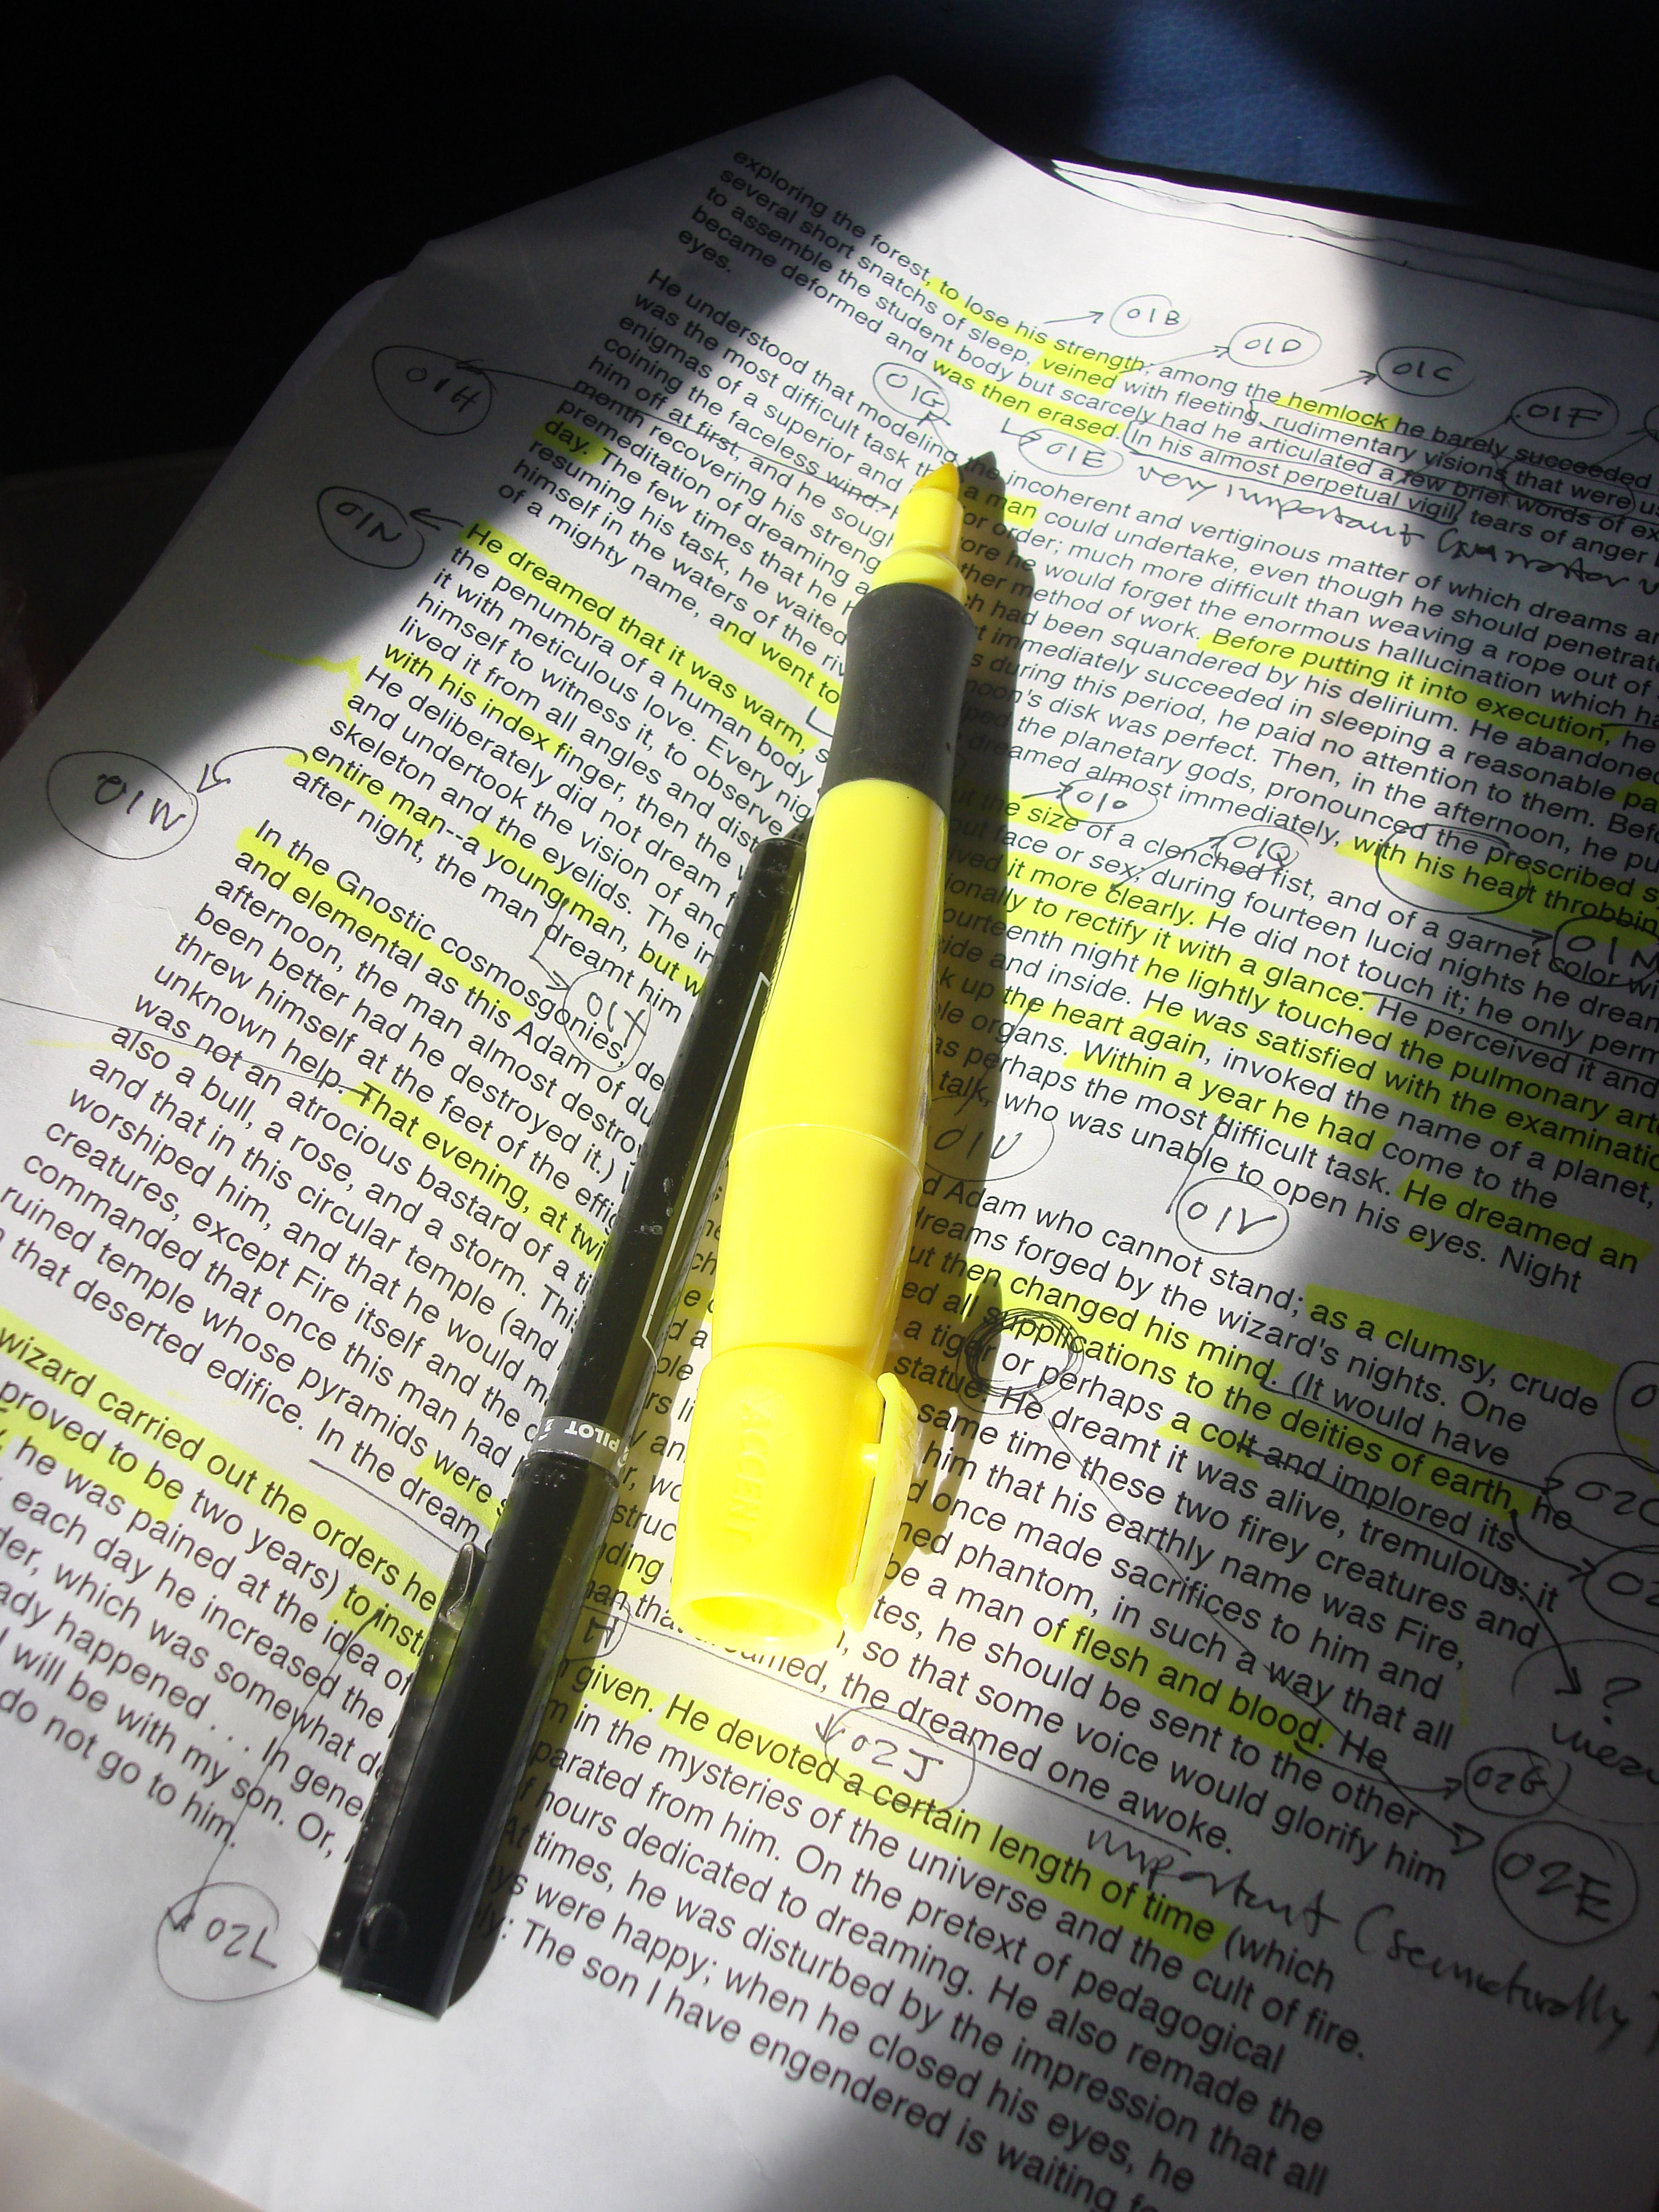
\includegraphics[width=\textwidth]{../img/textmarker}
  \end{columns}

  \vfill

  \hrulefill\\
  \hfill {\tiny Image by Guido ``random'' Alvarez, released as CC-BY-2.0}

\end{frame}

\subsection{Understanding the Input/Output}

\begin{frame}
  \frametitle{Task 2: Reading the Input/Output}
  The Input Description is \alert{very important} (as we saw in 3n+1)
  \bigskip

  \begin{itemize}
  \item What is the stop condition?
  \begin{itemize}
    \item The number of inputs is given in the beginning;
    \item Special value to indicate the end of the input;
    \item Input ends at the end of the file (EOF);
  \end{itemize}
  \medskip

  \item What is the format of the input/output?
  \begin{itemize}
    \item Very important for output (floating point precision)
  \end{itemize}
  \medskip

  \item What is the size of the input?
  \begin{itemize}
    \item What is the maximum number of inputs?
    \item What are the maximum and minimum values?
    \item Are there special conditions?
  \end{itemize}
  \end{itemize}
\end{frame}

\begin{frame}
  \frametitle{Task 2: Estimate time limit from input size}

  The input size shows how big the problem gets.

  \begin{itemize}
    \item Small Problem: You can use brute force algorithms;
    \item Big Problem: You need to use more complex algorithms; Maybe \alert{prune} the input;
  \end{itemize}
  \bigskip

  \begin{block}{Estimate the "Time Limit Exceeded" limit}
    \begin{itemize}
    \item expect around 10,000,000 operations per second on the online judge;
    \item most problems have 1-3 seconds of time limit;
    \item python can be a bit slower!
    \end{itemize}
  \end{block}
\end{frame}

\begin{frame}{Task 2: Input size examples}

  \begin{block}{n $<$ 24}
    Exponential algorithms will work (O($2^n$)).\\
    Or sometimes you can just calculate all solutions.
  \end{block}

  \begin{block}{n = 500}
    Cubic algorithms don't work anymore (O($n^3$) = 125.000.000)\\
    Maybe O($n^2\text{log}n$) will still work.
  \end{block}

  \begin{block}{n = 10.000}
    A square algorithm (O($n^2$)) might still work.\\
    But beware any big constants!
  \end{block}

  \begin{block}{n = 1.000.000}
    O($n$log$n$) = 13.000.000\\
    We might need a linear algorithm!
  \end{block}
\end{frame}

\begin{frame}
  \frametitle{Task 2: Input Format}

  Three common patterns for input format:
  \vfill

  \begin{itemize}
  \item Read $N$, then read $N$ queries;
  \bigskip

  \item Read until a special condition;
  \bigskip

  \item Read until EOF;
  \end{itemize}
\end{frame}

\begin{frame}[fragile]
  \frametitle{Task 2: Input Format}
  \begin{block}{}
    Read $N$, and then read $N$ queries;
    \bigskip

    Remember $N$ when calculating the size of the problem!
  \end{block}
  Example: \structure{Cost Cutting}

{\smaller
\begin{verbatim}
#include <iostream>
using namespace std;

int main()
{
    int n;
    cin >> n;

    for (; n > 0; n--)
    {
       // Do something
    }
}
\end{verbatim}}

\end{frame}

\begin{frame}[fragile]
  \frametitle{Task 2: Input Format}
  \begin{block}{}
    Read Until a Special Condition.

    Be careful: You can have \alert{many} queries before the condition!
  \end{block}

  Example: \structure{Request for Proposal:}\\
  The input ends with a line containing two zeroes.

{\smaller
\begin{verbatim}
int main()
{
   cin >> n >> p;
   while (n!=0 || p!=0)
   {
       // do something!
       cin >> n >> p;
   }
}
\end{verbatim}}
\end{frame}

\begin{frame}[fragile]
  \frametitle{Task 2: Input Format}
  \begin{block}{}
    Read until EOF.
    \bigskip

    Functions in C and Java return FALSE when they read EOF. Python requires
    an exception. Very common in UVA.
  \end{block}
  Example: \structure{3N+1 Problem, Jolly Jumpers}

{\smaller
\begin{verbatim}
int main()
{
    int a, b;
    while (cin >> a >> b;)
    {
        // Do something!
    }
}
\end{verbatim}
}
\end{frame}

\begin{frame}
  \frametitle{Task 2: Output Format}

  The UVA judge decides the result based on a simple \alert{diff}.
  \bigskip

  Be \alert{very careful} that the output is exactly right!

  \vspace{3cm}

  \begin{columns}
    \column{0.2\textwidth}
    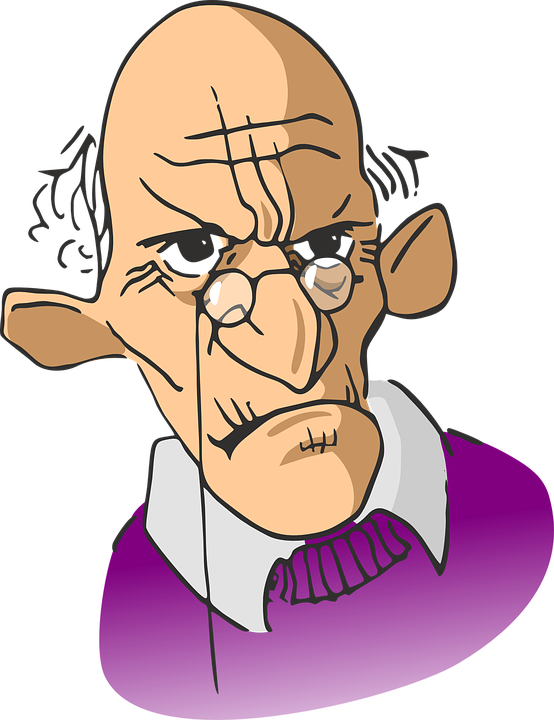
\includegraphics[width=1\textwidth]{../img/angryclient}
    \column{0.7\textwidth} \emph{The Judge is like an angry client. It
      wants the output EXACTLY how it stated.}
  \end{columns}
\end{frame}

\begin{frame}
  \frametitle{Task 2: Output Format -- Checklist}

  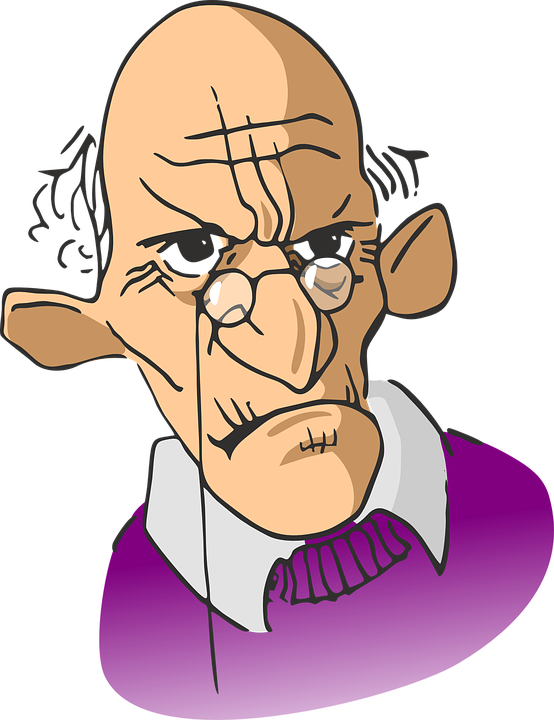
\includegraphics[width=0.15\textwidth]{../img/angryclient}
  \begin{enumerate}
    \item DID YOU REMOVE DEBUG OUTPUT?
    \item DID YOU REMOVE DEBUG OUTPUT?
    \smallskip

    \item Easy mistakes: UPPERCASE x lowercase, spleling mitsakes;
    \item Boring mistakes: plural: 1 hour \structure{or} 2 hours;
    \item What is the precision of \structure{float}? (3.051 \structure{or} 3.05)
    \item Round up or Round down? (3.62 $\rightarrow$ 3 \structure{or} 4)
    \item Multiple solutions: Which one do you output\\ (usually ortographical sort)
  \end{enumerate}
\end{frame}


\begin{frame}
  \frametitle{Task 2: Tricks in the input/output}

  \begin{block}{Example: 3n+1 Problem}
    \begin{itemize}
    \item $i$ and $j$ can come in any order.
    \end{itemize}
  \end{block}

  \begin{block}{Common Traps}
    \begin{itemize}
    \item Negative numbers, zeros;
    \item Duplicated input, empty input;
    \item No solutions, multiple solutions;
    \item Other special cases;
    \end{itemize}
  \end{block}
  \vfill

  \hfill 
\includegraphics[width=0.25\textwidth]{../img/trap}
\end{frame}

\subsection{Task 3: Choosing the algorithm}


\begin{frame}
  \frametitle{Task 3: Choosing the algorithm}
  The important part of choosing the algorithm is \alert{counting the time}
  \bigskip

  \begin{itemize}
    \item An algorithm with $k$-nested loops of and $n$ commands
      has $O(nk)$ complexity;
    \item A recursive algorithm with $b$ recursive calls per level, and $L$
      levels, it should have $O(bL)$ complexity;
    \item An algorithm with $p$ nested loops of size $n$ is $O(n^p)$
    \item An algorithm processing a $n*n$ matrix in O(k) per cell runs
      in $O(kn^2)$ time.
  \end{itemize}
  \bigskip

  One way to reduce the cost of a program is to use \alert{pruning}
\end{frame}

\begin{frame}{Task 3: Example of Pruning -- 8 queen problem}

  \alert{Pruning} is when you quickly remove bad cases to reduce the
  computational cost of an algorithm.
  \bigskip

  The "8-queens" problem is a good problem to understand pruning. We
  want to find all possible positions of 8 queens in a chessboard,
  where they don't attack each other.
  \bigskip

  The brute force algorithm is: Try all possible positions, and check if
  they are valid. \alert{But how we list all positions make a big difference}.

  \hfill 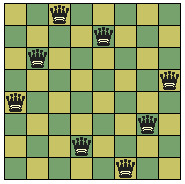
\includegraphics[width=0.2\textwidth]{img/8queen}
\end{frame}

\begin{frame}[fragile]{Task 3: Example of Pruning -- 8 queen problem}{Approach 1 -- all squares}

  \hfill 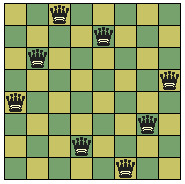
\includegraphics[width=0.2\textwidth]{img/8queen}

  Approach 1: For each queen, test all possible squares;
  \bigskip

\begin{verbatim}
Queen1: a1 or a2 or a3 or a4 ... or h5 or h6 or h7 or h8
Queen2: Same as Queen 1
Queen3: Same as Queen 2
...
Queen8: Same as Queen 7

Total Solutions: 64 x 64 x 64 x 64 = 64^8 ~ 10^14
\end{verbatim}
\end{frame}

\begin{frame}[fragile]{Task 3: Example of Pruning -- 8 queen problem}{Approach 2 -- columns}

  \hfill 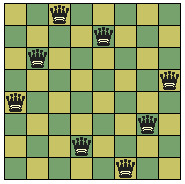
\includegraphics[width=0.2\textwidth]{img/8queen}\\
  Approach 2: Choose one column for each queen, test all rows.
  \bigskip

\begin{verbatim}
Queen1: a1 or a2 or a3 ...
Queen2: b1 or b2 or b3 ...
Queen3: c1 or c2 or c3 ...
...
Queen8: h1 or h2 or h3 ...

Total Solutions: 8 x 8 x 8 ... = 8^8 ~ 10^7
\end{verbatim}
\end{frame}

\begin{frame}[fragile]{Task 3: Example of Pruning -- 8 queen problem}{Approach 3 -- permutation}

  \hfill 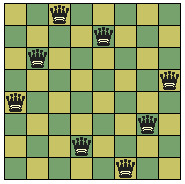
\includegraphics[width=0.2\textwidth]{img/8queen}\\
  Choose one column for each queen, test a row not used.
  \bigskip

\begin{verbatim}
If Q1 is a1, Q2 in b2, Q3 must be c3-7...

A solution is the order of rows: Ex: 1-3-5-2-7-4-8-6

Total Solutions: 8 x 7 x 6 x 5 ... = 40320
\end{verbatim}
\end{frame}

\begin{frame}{Task 3: Example of Pruning -- 8 queen problem}{Pruning comparison}

  \hfill 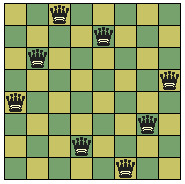
\includegraphics[width=0.2\textwidth]{img/8queen}
  \begin{itemize}
    \item Approach 1: All rows and columns: $10^{14}$ steps;
    \item Approach 2: All rows: $10^{7}$ steps;
    \item Approach 3: Permutation: 40320 steps;
  \end{itemize}
  \bigskip

  Same algorithm (brute force), but pruning changes the efficiency!
\end{frame}

\subsection{Task 4: Coding}

\begin{frame}
  \frametitle{Task 4: Coding}

  After you understand what the problem requires you to do, and after you decide which algorithm to use, then you can begin programming.
  \bigskip

  Avoid beging programming before you have a good idea of what you are going to do. Early programming might lead to bugs, and you may decide that you want to change your algorithm or data structure;
\end{frame}

\begin{frame}
  \frametitle{Hints when coding}
  \begin{exampleblock}{Hint 1: Coding Library}
    As you solve many programs, save functions and patterns that you use many times:
    \begin{itemize}
    \item Code for different types of Input;
    \item Common data structures;
    \item Difficult algorithms;
    \end{itemize}
   \end{exampleblock}

   \begin{block}{Hint 2: Use paper}
    When you write your idea on paper (diagrams, code), it helps you clarify parts that are not well defined in your mind.
    \medskip

    Sometimes this helps you find problems in your idea early.
  \end{block}
\end{frame}

\begin{frame}
  \frametitle{Hints when Coding}

  \begin{block}{Hint 3: "Programmer Efficiency"}
    We often think about {\bf CPU efficiency} (program is fast), or {\bf memory efficiency} (program uses little memory).
    \bigskip

    But another very important efficiency is {\bf Programmer Efficiency}: If the program is too complex, the programmer will get tired or confused!
    \begin{itemize}
      \item Complex programs take longer to complete;
      \item Complex programs are harder to debug;
      \item You can't reuse code from complex programs easily;
    \end{itemize}
  \end{block}
  How to improve programmer efficiency:
  \begin{itemize}
  \item Learn and use the standard library and macros;
  \item Create your own library of programming challenge patterns;
  \item Focus on the minimal features for this problem;
  \item Use clear names for variables and functions;
  \end{itemize}
\end{frame}


\subsection{Task 5: Testing}
\begin{frame}
  \frametitle{Sample data and Hidden Data}
  Remember that the sample data in the program is not all data! The Online Judge will use a set of {\bf hidden data}.
  \bigskip

  Generate your own set of data to test your program before submitting.
  \bigskip

  \begin{columns}
    \column{0.45\textwidth}
    \begin{exampleblock}{Sample Data}
      \begin{itemize}
      \item Useful to test the input/output functions;
      \item You can read the sample data to understand the problem;
      \item Does NOT include tricky cases;
      \end{itemize}
    \end{exampleblock}
    \column{0.45\textwidth}
    \begin{alertblock}{Hidden Data}
      \begin{itemize}
      \item Data of the online judge;
      \item Much bigger cases, uses maximum and minimum values;
      \item Data includes tricky cases and worst cases;
      \end{itemize}
    \end{alertblock}
  \end{columns}
\end{frame}

\begin{frame}
  \frametitle{Generating testing data cases}
  "Be mean. Generate data that will show bugs in your program, not data
  that you expect to work."

  \begin{itemize}
  \item Repeat one case many times in the same file (check for initialization);
  \item Random data with maximum size/values (test for array limits and general performance);
  \item Border cases (maximum and minimum values);
  \item Worst cases (what data would make the algorithm run slowest? If you don't know the worst case, maybe you don't understand the algorithm yet!);
  \end{itemize}
  \bigskip

  In particular for random and large test data sets, I recommend that you create a simple script that generates random data for you. Random data is great for finding "crash" bugs.
\end{frame}

\begin{frame}
  \frametitle{Test data website: uDebug}
  The udebug website \url{https://www.udebug.com/} has test cases for many problems in online-judge. \alert{However, note that it does not necessarily has all test cases}!
  \bigskip

  \begin{center}
    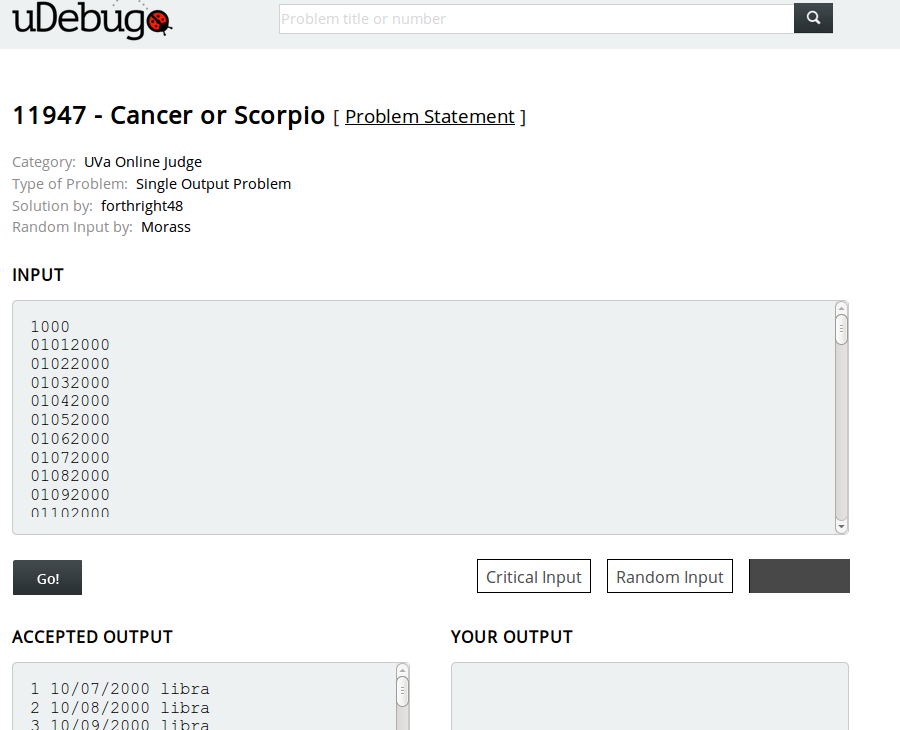
\includegraphics[width=0.8\textwidth]{../img/udebug_big}
  \end{center}
\end{frame}

\section{Conclusion}
\subsection{The End}
\begin{frame}
  \frametitle{To Summarize}
  Mental framework to solve problems:
  \begin{enumerate}
  \item Read the problem carefully to avoid traps;
  \item Think of the algorithm and data structure;
  \item Keep the size of the problem in mind;
  \item Keep your code simple;
  \item Create special test cases;
  \end{enumerate}

  \vfill

  \begin{block}{}
    Now go solve the other problems!
  \end{block}
\end{frame}

\begin{frame}
  \frametitle{Thanks for Listening!}
  \begin{center}
    Send questions to the manaba forums!
  \end{center}
\end{frame}

% \begin{frame}
%   \frametitle{BONUS -- Calculating Complexity in Research Experiments}
% \end{frame}
%
% \begin{frame}
%   \frametitle{BONUS -- A very simple program}
%
%   \begin{block}{Ackermann's Function}
%     \begin{eqnarray*}
%       A(m,n) = & n+1 & \text{if } m = 0\\
%       & A(m-1,1) & \text{if } m > 0, n = 0\\
%       & A(m-1,A(m,n-1)) & \text{if } m > 0, n > 0\\
%     \end{eqnarray*}
%   \end{block}
%
%   \begin{itemize}
%     \item $A(0,n) = 1$ step
%     \item $A(1,n) = 2n+2$ steps
%     \item $A(2,n) = n^2$ steps
%     \item $A(3,n) = 2^{n+3}-3$ \alert{!}
%     \item $A(4,n) = 2^{2^{...^2}}-3$ \alert{!!!} (exponential tower of n+3)
%     \item $A(5,n) = $ \alert{!!!!!!!!!!!!}
%   \end{itemize}
%\end{frame}
